\documentclass[10pt]{article}
\usepackage[utf8]{inputenc}
\usepackage[T1]{fontenc}
\usepackage{amsmath}
\usepackage{amsfonts}
\usepackage{amssymb}
\usepackage[version=4]{mhchem}
\usepackage{stmaryrd}
\usepackage{graphicx}
\usepackage[export]{adjustbox}
\graphicspath{ {./images/} }

\begin{document}

    "Daksha" is a proposed Indian mission consisting of two satellites $\mathrm{S}_{1}$ and $\mathrm{S}_{2}$ orbiting the Earth in the same circular orbit of radius $r=7000 \mathrm{~km}$ but with $180^{\circ}$ phase difference. These satellites observe the universe in high energy domain (X-rays and $\gamma$-rays). Each of the satellites of Daksha uses several flat, rectangular detectors.

    To understand how to localize a source in the sky, we shall use a simplified model of the Daksha mission. Assume that $\mathrm{S}_{1}$ has only two identical detectors $\mathrm{D}_{1}$ and $\mathrm{D}_{2}$, each of area $A=0.50 \mathrm{~m}^{2}$, attached to an opaque mount M as shown in the figure below. The detectors lie symmetrically around the $y$-axis in planes perpendicular to the $x-y$ plane and make an angle $\alpha=120^{\circ}$ with each other.\\
    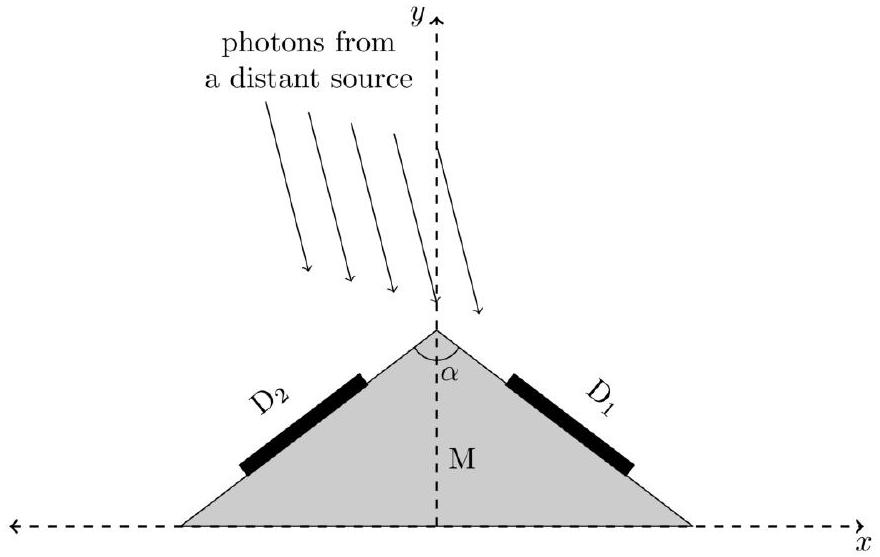
\includegraphics[max width=\textwidth, center]{2025_08_23_e94579452776a99c4850g-01}\\
    (T01.1) When observing a distant source located in the $x-y$ plane, detector $\mathrm{D}_{1}$ records a power $P_{1}= 2.70 \times 10^{-10} \mathrm{~J} \mathrm{~s}^{-1}$ and detector $\mathrm{D}_{2}$ records a power $P_{2}=4.70 \times 10^{-10} \mathrm{~J} \mathrm{~s}^{-1}$.
    
    Estimate the angle $\eta$ made by the position vector of the source with the positive $y$-axis, with counter-clockwise angle from the positive $y$-axis being considered positive.
    
    Consider a single pulse from a distant source (not necessarily in the $x-y$ plane) recorded by both satellites ( $\mathrm{S}_{1}$ and $\mathrm{S}_{2}$ ) of Daksha. The times of the peaks of the pulses recorded by $\mathrm{S}_{1}$ and $\mathrm{S}_{2}$ are $t_{1}$ and $t_{2}$, respectively.\\
    (T01.2) If $t_{1}-t_{2}$ was measured to be $10.0 \pm 0.1 \mathrm{~ms}$ then determine the fraction, $f$, of the celestial sphere where the source might lie.

\end{document}